\section{Approach}
\label{s:approach}
%Approach; What selection of deep uncertainty methods are you using, in what order, and why? This should be clearly motivated and grounded in the literature

% Analysis is carried out across the explicated rival problem framings and relies on state-of- the-art deep uncertainty techniques

% Analysis is carried out across the explicated rival problem framings and relies on state-of- the-art deep uncertainty techniques
We considered multiple alternative approaches to analyse the explicated problem framings. Ultimately, we adopted a straightforward combination of techniques to analyse and interpret the problem framings of Gorssel, as well as its two rival/coalition-forming actors, Deventer and Overijssel. Ultimately, we chose a multi-scenario multi-objective robust decision-making (MORDM) process to analyse and select policy approaches. We chose this approach for its ability to achieve a balance between finding robust solutions that are optimal in specific scenarios while also being computationally efficient, given constraints in time and computing power \parencite{bartholomew_considering_2020}. A visualisation of the workflow we adopted is shown in Figure~\ref{fig:msmordm}. Below, we explain the deep uncertainty techniques applied in each step and selections of these approaches motivated in light of currently available literature. 

\begin{figure}[h]
    \centering
    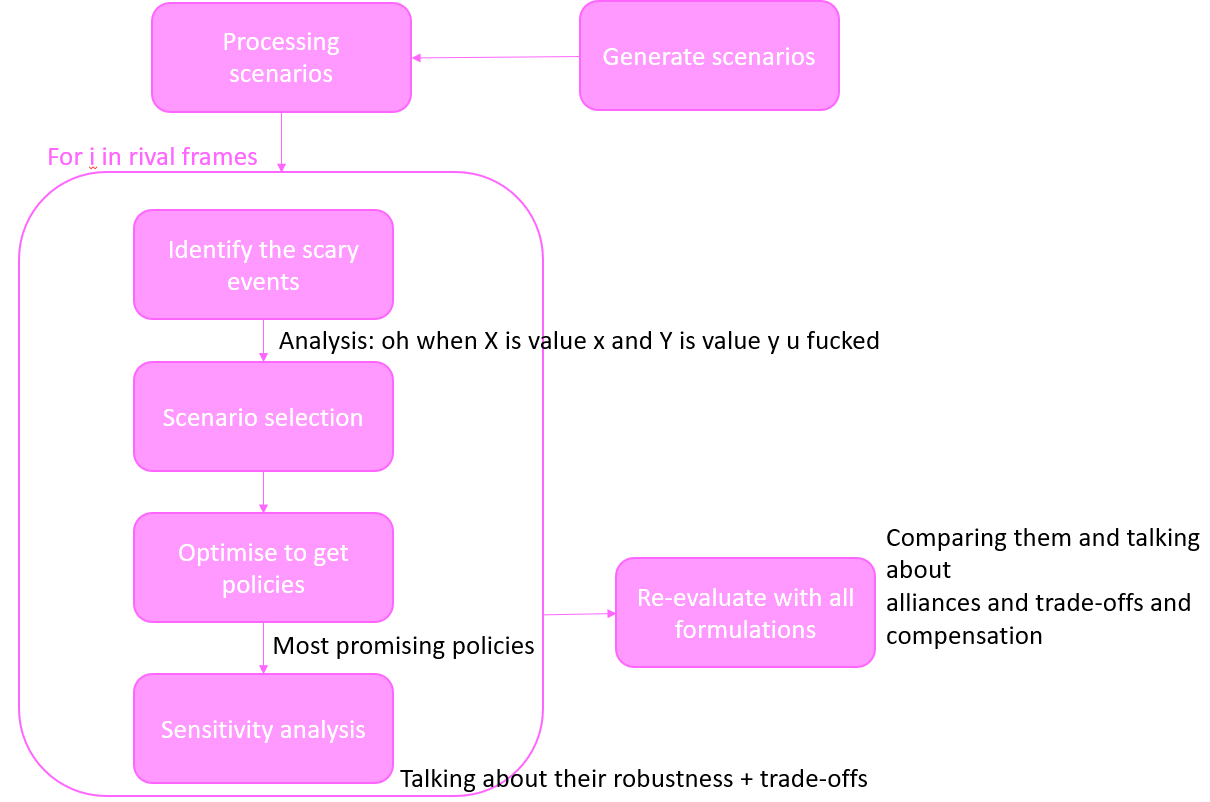
\includegraphics[width=0.8\textwidth]{report/figures/methodology.png}
    \caption{The MSMORDM Process, inspired by  \citeauthor{bartholomew_considering_2020}}
    \label{fig:msmordm}
\end{figure}

We used the Exploratory Modelling Workbench (an open-source Python library) to implement this approach ~\parencite{kwakkel_exploratory_2017}. Readers can find Jupyter Notebooks and Python files for the reproduction of the analysis implementation in the repository in the Appendix~\ref{s:repository}.

%In what order are we using the tools, and why are we using them this way
\subsection{Problem Formulation}
In the first step of this process, we defined the problem formulations for each of the three actors, as described in Section \ref{s:prob_frame}. For each actor, we defined multiple objectives to elicit relevant trade-offs (predominantly between cost and risk). We used these formulations to initialise the model to run experiments. We opted to look at results over three planning steps (each step equates to roughly 67 years) to observe the evolution of planning and risk and get more granularity in the potential policies and uncertainties.

\subsection{Generation of Scenarios}
For the experiments, we generated 50,000 scenarios for each actor (without policies). We chose to run 50,000 scenarios for each actor to trade off the granularity/resolution of available scenarios against the computational intensity of generating and optimising over this large range. A large number of scenarios was also necessary as the chosen problem framing increased the number of uncertainties in the model (that is, the levers for actors outside of Overijssel Province). We opted to use the LHS uncertainty sampling method, which splits the uncertainty space into intervals of equal probability.

We also modified the underlying model to serve the selected problem formulation by disaggregating the cost factors of Room for the River Costs and the Evacuations Costs, such that costs for the actors of Gorssel and Deventer were individualised. The ranges of the uncertainties already present in the model were left unchanged. We also used the population size for Deventer and Lochem to get the difference in damage in deaths per capita. 


\subsection{Sensitivity Analysis and Scenario Discovery}
Since no policies were implemented, all costs were 0, so we could disregard this outcome for now. We also performed a quick data inspection and found a high correlation between deaths and damages for all actors: $0.98$ for Gorssel, $0.98$ for Deventer, and $0.98$ for Overijssel. Hence, for the remainder of this step of the analysis, we primarily focused on damage.

Following this, we conducted sensitivity analysis and scenario discovery to identify the most dominant uncertainties and levers in the input space for each of the three actors (regarding damage). For Uncertainty analysis, we employed the Extra Trees algorithm. It showed that for Gorssel, only the durability of their own dike was by far the most dominant (estimator instance of 0.56). For Deventer and Overijssel, Deventer's dike durability was the most dominant (estimator instances of 0.45 and 0.55, respectively). All other uncertainties and levers had an estimator instance $<0.081$. All estimator instances can be seen in Appendix~\ref{a:sensitivity-analysis}.

We conducted scenario discovery using the PRIM algorithm, as it allowed us to visualise and investigate the uncertainty space to identify suitable ranges of uncertainty for scenario selection in the multi-scenario MORDM process \parencite{bryant_thinking_2010}. We specifically looked at the worst 10th percentile of damages and the best 40th percentile. Whenever a density $\rho$ with $\rho>0.8$ was reached, we looked at the range of uncertainties. This showed that the durability of Gorssel's dike is also dominant for Overijssel (even though it had an estimator instance of 0.06 during the sensitivity analysis).

This process thus revealed that the most dominant uncertainties for the three actors were the probability of dike failure at either Gorssel and/or Deventer. These factors were the strongest determinants of policy success across the broadest range of scenarios. These uncertainties and their influence on the worst 10th percentile and best 40th percentile is shown in Figure~\ref{fig:prim}.

\subsection{Scenario Selection}
Provided this information on the importance of different uncertainties on outcomes of interest, we developed a process for selecting six scenarios over which the model could develop policies. We gave attention to ensure a good distribution of dike failure probability values across the selected scenarios. We opted for a mixture of good, 'middle', and worst-case scenarios to enable us to observe the performance of and preferences towards policies under the broadest range of scenarios. We also did this to support stakeholder comprehension of policy outcomes. The logic used to select the scenarios is shown in Table~\ref{tab:scenarios}. The best scenario was just one of the scenarios that resulted in 0 deaths and damages. The worst deaths and worst damage scenarios were the scenarios that resulted in most deaths or damage, respectively. The absolute worst scenario is the scenario with the combined highest damage and deaths. For all actors, this scenario was the same as either the worst damage (for Gorssel) or worst deaths (Overijssel and Deventer), in which we opted to continue with the "absolute worst" label for that scenario. This means that the scenario with most damage was always a different scenario than the one with the most deaths. We selected the remaining scenarios based on the union of the scenarios present in the ranges displayed in the table. Note that we needed to use a more extensive range for Deventer's low scenario, which means there is less correlation in the lower range of Deaths and Damages.

\begin{table}[h!]
\caption{A crude notation of the logic that we used to select scenarios. We applied these ranges to both Damage and Deaths for low, middle and high, and the scenario would have to be present in both. Deventer's low scenario range is bigger, as there is less overlap between the two outcomes than for the other actors. We just picked a scenario with 0 deaths and 0 damages for the best scenario, and for the worst scenarios, we just picked the scenarios with the worst outcomes. For all actors, either worst damage or worst deaths was the same as the absolute worst scenario, hence why either one of these is excluded (indicated with an \emph{x}) from the set of scenarios. The absolute worst was selected by normalising Damages and deaths and dividing it by 2, meaning that if damages and deaths were highest in the same scenario, this value would equal 1.}
\label{tab:scenarios}
\centering
\begin{tabular}{lccc}
               & Gorssel& Deventer & Overijssel \\
best           & $D_1 = 0 \land D_2 = 0$ & $D_1 = 0 \land D_2 = 0$ & $D_1 = 0 \land D_2 = 0$ \\
low            & $23\%> D \leq 27\% $ & $25\%> D \leq 35\%$ & $23\%> D \leq 27\%$\\
middle         & $48\%> D \leq 52\%$ & $48\%> D \leq 52\%$ & $48\%> D \leq 52\%$ \\
high           & $73\%> D \leq 77\%$ & $73\%> D \leq 77\%$ & $73\%> D \leq 77\%$            \\
worst deaths   & $max(D_1)$ & x & x \\
worst damage   & x & $max(D_2)$ & $max(D_2)$ \\
absolute worst & $max(\frac{norm(D_1)+norm(D_2)}{2}) $ & $max(\frac{norm(D_1)+norm(D_2)}{2})$ & $max(\frac{norm(D_1)+norm(D_2)}{2})$           
\end{tabular}
\end{table}

The two 'worst case' scenarios (one representing worst case for deaths or damages, and another across all outcomes) exist within the uncertainty range for the probability of failure identified in the previous step. This is shown in Figure~\ref{fig:prim}.

\begin{figure}[h]
    \centering
    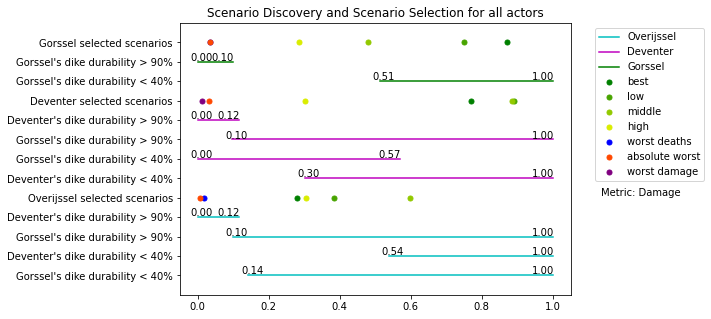
\includegraphics[width=\textwidth]{report/figures/results/scenario_discovery.png}
    \caption{The results from the scenario discovery process and the selected scenarios. The first three items in the legend are the actors, and the remaining items are the scenarios. $<40\%$ is all the scenarios with damage up to the 40th percentile, and $>90$ are all the scenarios that have damage between the 90th and 100th percentile. All values of the dominant uncertainties of the "worst scenarios" correspond to the worst 10th percentile.}
    \label{fig:prim}
\end{figure}

\noindent We selected this approach instead of a 'maximise diversity' approach due to time constraints in the computational intensity of such an approach over such a large number of scenarios and uncertainties \parencite{eker_including_2018}.

\subsection{Identifying Policy Alternatives}

Following scenario generation, we generated policy alternatives by optimising the policy objectives for the three actors to determine the Pareto-approximate set, using a many-objective evolutionary algorithm. The algorithm used was $\epsilon$-NSGA2. We considered this algorithm appropriate for our formulations, as previous studies have shown that it performs well for six-objective problem formulations in related applications \parencite{salazar_diagnostic_2016}. The epsilon values for these optimisations were selected through trial and error, informed by the range of values observed in the generated scenarios, with attention given to the number of potential policies generated from each iteration. We were ultimately satisfied that the chosen epsilon values represented an optimisation space that could trade-off between generating a sufficient number of interesting policy combinations without creating so much granularity that there was duplication or 'nonsense' policies being generated. The number of function evaluations for each optimisation were also selected based on trial and error, with the optimisations re-run until model results converged.

\subsection{Re-evaluation of Policies under Deep Uncertainty and Subset Selection}
Having selected these six scenarios over which to optimise, we ran the Many-Objective Evolutionary Algorithm (MOEA) to identify Pareto-approximate policies for each scenario for each actor. Then we discarded duplicate policies and selected a more manageable subset by clustering the remaining subset with k-means (with $K=6$) to get 6 clusters. Within those clusters, we normalised the lever values and summed the values per policy. Then we selected the policies with the highest two sums to get the most "extreme" policies per cluster. This means that there were at most 12 different policies to be processed by the next step.

\subsection{Robustness Analysis}
We then examined the subsetted selection of policy alternatives according to two types of robustness metrics: one satisficing and one regret based (domain-criterion \parencite{bartholomew_considering_2020}). We considered the use of two metrics necessary to see where there might be disagreement between the two types of metrics and to identify if any policies achieve good scores under both metrics (indicating policies that are more robust across different perspectives) \parencite{mcphail_robustness_2018}. These robustness metrics then resulted in a final shortlist of five candidate policies per actor.

Readers can find the threshold values for the satisficing analysis in \autoref{tab:threshold}. The threshold values for the total costs are the exact budgets of the institutions for water/traffic management so that it is a somewhat realistic representation. We set expected annual damage as 10\% of the Total costs available every year to the institutions. We calculated the values for expected annual deaths from the maximum risk of 1:100,000 people that can die from flooding multiplied \parencite{slootjes_achtergronden_2016}, which we then multiplied with the population of the area.


\begin{table}[H]
\centering
\caption{This table shows the threshold values for the three actors. The values for the town of Gorssel come from its bigger municipality Lochem \parencite{gemeente_lochem_programmabegroting_nodate}. Deventer's value is derived from \parencite{gemeente_deventer_leefomgeving_nodate}. The value for Overijssel is obtianed from \parencite{provincie_overijssel_begroting_nodate}}
\label{tab:threshold}
\begin{tabular}{@{}llll@{}}
\cmidrule(l){2-4}
 &
  \multicolumn{3}{c}{\textbf{Robustness Threshold Values}} \\ \cmidrule(l){2-4} 
\multicolumn{1}{l|}{} &
  \multicolumn{1}{l|}{\textbf{Outcome}} &
  \multicolumn{1}{l|}{\textbf{Goal}} &
  \multicolumn{1}{l|}{\textbf{Threshold}} \\ \cmidrule(l){2-4} 
\multicolumn{1}{c|}{\multirow{3}{*}{Gorssel}} &
  \multicolumn{1}{l|}{\begin{tabular}[c]{@{}l@{}}Expected annual\\ damage\end{tabular}} &
  \multicolumn{1}{l|}{Minimize} &
  \multicolumn{1}{l|}{$5.4E+05$} \\ \cmidrule(l){2-4} 
\multicolumn{1}{c|}{} &
  \multicolumn{1}{l|}{\begin{tabular}[c]{@{}l@{}}Expected annual\\ casualties\end{tabular}} &
  \multicolumn{1}{l|}{Minimize} &
  \multicolumn{1}{l|}{$1.0E-05$} \\ \cmidrule(l){2-4} 
\multicolumn{1}{c|}{} &
  \multicolumn{1}{l|}{Total costs} &
  \multicolumn{1}{l|}{Minimize} &
  \multicolumn{1}{l|}{$5.4E+06$} \\ \cmidrule(l){2-4} 
\multicolumn{4}{l}{} \\ \cmidrule(l){2-4} 
\multicolumn{1}{l|}{\multirow{3}{*}{Deventer}} &
  \multicolumn{1}{l|}{\begin{tabular}[c]{@{}l@{}}Expected annual\\ damage\end{tabular}} &
  \multicolumn{1}{l|}{Minimize} &
  \multicolumn{1}{l|}{$1.1E+06$} \\ \cmidrule(l){2-4} 
\multicolumn{1}{l|}{} &
  \multicolumn{1}{l|}{\begin{tabular}[c]{@{}l@{}}Expected annual\\ casualties\end{tabular}} &
  \multicolumn{1}{l|}{Minimize} &
  \multicolumn{1}{l|}{$1.0E-05$} \\ \cmidrule(l){2-4} 
\multicolumn{1}{l|}{} &
  \multicolumn{1}{l|}{Total costs} &
  \multicolumn{1}{l|}{Minimize} &
  \multicolumn{1}{l|}{$1.1E+07$} \\ \cmidrule(l){2-4} 
\multicolumn{4}{l}{} \\ \cmidrule(l){2-4} 
\multicolumn{1}{l|}{\multirow{3}{*}{Overijssel}} &
  \multicolumn{1}{l|}{\begin{tabular}[c]{@{}l@{}}Expected annual\\ damage\end{tabular}} &
  \multicolumn{1}{l|}{Minimize} &
  \multicolumn{1}{l|}{$1.53E+06$} \\ \cmidrule(l){2-4} 
\multicolumn{1}{l|}{} &
  \multicolumn{1}{l|}{\begin{tabular}[c]{@{}l@{}}Expected annual\\ casualties\end{tabular}} &
  \multicolumn{1}{l|}{Minimize} &
  \multicolumn{1}{l|}{$1.0E-05$} \\ \cmidrule(l){2-4} 
\multicolumn{1}{l|}{} &
  \multicolumn{1}{l|}{Total costs} &
  \multicolumn{1}{l|}{Minimize} &
  \multicolumn{1}{l|}{$1.53E+07$} \\ \cmidrule(l){2-4} 
\end{tabular}
\end{table}

\subsection{Uncertainty Analysis}
\label{ss:sensitivity-analysis}
We then assessed the candidate policies for each actor for their sensitivity to uncertainties. The chosen method for global uncertainty analysis was the Extra Trees algorithm. We chose this approach as it is known to be an effective means of replicating the insights of global uncertainty analysis with much lower computational requirements \parencite{jaxa-rozen_tree-based_2018}.

\subsection{Policy Synthesis}
Finally, we ran Gorssel's policies for Overijssel's to see how receptive Overijssel is to Gorssel's optimal policies, and we used the approaches from Deventer and Overijssel and ran them for Gorssel's objective to see how good/bad they are for our client. 
Additionally, we identified where there are policies that are consistent (or at least similar) between actors to support coalition forming (in the case of consistent policies) or informing policy negotiations (in the case of inconsistent policies). We compared the five candidate policies from each actor to find potential similarities in lever choices, informing opportunities for coalition-building or areas for negotiation in future formulations and iterations over the multi-scenario MORDM process.



